\chapter*{Introducción}
 
El artículo de Claude Shannon \textit{Mathematical Theory of Cryptography} \parencite{shannon_mathematical_1945} y su ampliación posterior, \textit{Mathematical Theory of Communication} \parencite{shannon_mathematical_1948} dieron a luz a dos disciplinas hoy plenamente establecidas, la teoría de información y la teoría de códigos.
El objetivo principal de estas disciplinas es el de establecer mecanismos de comunicación que sean \emph{eficientes} y \emph{fiables} en ambientes posiblemente hostiles.
La eficiencia requiere que la transmisión de la información no necesite de demasiados recursos, sean materiales o temporales.
Por otro lado, la fiabilidad requiere que el mensaje recibido en una comunicación sea lo más parecido posible, dentro de unos márgenes de tolerancia, al mensaje original.
La teoría de la información se encarga del estudio tanto de la representación de la información como de la capacidad que tienen los sistemas para transmitir y procesar la información. 
Por otra parte, la teoría de códigos se basa en los resultados de la teoría de la información para el diseño y desarrollo de modelos de transmisión de información mediante herramientas algebraicas.

A pesar de que digamos que Shannon fue el padre de estas disciplinas, el problema de codificar la información no surge, ni mucho menos, entonces.
De hecho, el filósofo inglés Francis Bacon ya afirmó en el año 1623 que únicamente son necesarios dos símbolos para codificar toda la comunicación.
\blockquote[{\cite[30]{dyson_catedral_2015}}]{La transposición de dos letras en cinco emplazamientos bastará para dar 32 diferencias [y] por este arte se abre un camino por el que un hombre puede expresar y señalar las intenciones de su mente, a un lugar situado a cualquier distancia, mediante objetos ... capaces solo de una doble diferencia.}
Efectivamente, hoy en día la codificación binaria forma parte de prácticamente todos los aspectos nuestras vidas.

Sin embargo, el problema más relevante —y el que nos ocupa— es el de codificar la información para que se produzca una correcta transmisión y recepción de los mensajes a través de un canal.
Como parte de su teoría Shannon introdujo lo que posteriormente se conocería como \emph{modelo de comunicación} de Shannon, un esquema simplificado de cómo se produce la transmisión de información entre emisor y receptor a través de un canal.
\begin{figure}
  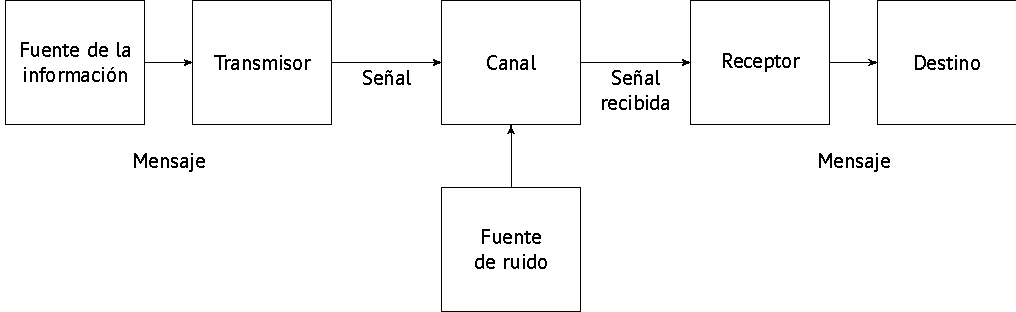
\includegraphics[width=\textwidth]{assets/shannon-communication-model.pdf}
  \caption*{Modelo de comunicación de Shannon}
\end{figure}
Al enviar la información a través del canal es posible que, debido al ruido que pueda haber en el mismo, se produzcan interferencias que alteren el mensaje enviado.
Por supuesto recibir un mensaje alterado no es deseable, pues es posible que la alteración sea tal que sea ilegible.
La teoría de códigos trata por tanto de diseñar estructuras algebraicas que permitan la corrección de errores por parte del receptor del mensaje.
Estas estructuras son los códigos, y son el objeto matemático sobre el que orbita todo este trabajo.


\section*{Enfoque}

El título de este trabajo es «Algoritmo de Peterson-Gorenstein-Zierler para códigos cíclicos sesgados», y como tal, expresa el objetivo último del mismo: estudiar y exponer este algoritmo.
En consecuencia, dirigiremos nuestra atención a los conceptos y herramientas necesarios para ello.
En cuanto a los fundamentos matemáticos necesarios, hablaremos de cuerpos finitos, anillos de polinomios sobre cuerpos finitos y anillos de polinomios de Ore sobre cuerpos finitos.
La teoría de códigos se centrará en la exposición de los códigos lineales y de los códigos cíclicos, así como de las familias de códigos concretas sobre las que trabajarán los algoritmos que vamos a describir.
Para comprender mejor el citado algoritmo estudiaremos también la versión original, de mitad del siglo pasado, para los conocidos como códigos BCH.
A lo largo del trabajo ilustraremos algunos ejemplos con el sistema algebraico computacional SageMath \parencite{the_sage_developers_sagemath_2020}.

\section*{Motivación}

Los códigos cíclicos son muy utilizados porque son muy sencillos de implementar en sistemas digitales utilizando lo que se conoce como registros de desplazamiento.
El uso de anillos de polinomios de Ore nos permite obtener una mayor cantidad de códigos cíclicos.
El algoritmo Peterson-Gorenstein-Zierler para códigos BCH es interesante porque es el que, en general, tiene un menor coste computacional para un número de errores pequeño.
La adaptación para códigos cíclicos sesgados ofrece.

\section*{Objetivos}

Los objetivos de este trabajo son los siguientes. \begin{itemize}
  \item Estudio de las nociones básicas sobre Teoría de Códigos lineales.
  \item Estudio de las extensiones de Ore y de sus cocientes.
  \item Exponer el algoritmo de Peterson-Gorenstein-Zierler para códigos cíclicos sesgados.
  \item Implementación de sistemas de decodificación en Python usando SageMath.
\end{itemize}

\section*{Esquema}

En los tres primeros capítulos introduciremos todos los fundamentos matemáticos necesarios, así como las definiciones y propiedades fundamentales de los códigos lineales y de los códigos cíclicos.
El capítulo cuarto ahondaremos en la familia de los códigos BCH y presentaremos el algoritmo original de Peterson-Gorenstein-Zierler para esta familia de códigos.
En el capítulo quinto explicamos las estructuras matemáticas que constituyen la base de los códigos cíclicos sesgados, los anillos de polinomios de Ore, para ya introducirlos propiamente en el capítulo sexto.
Finalmente, en el capítulo séptimo describimos el funcionamiento del algoritmo de Peterson-Gorenstein-Zierler para códigos cíclicos sesgados.



